% Diagrama conmutativo de equivarianza
% Compilar con: pdflatex equivariance_diagram.tex
\documentclass[tikz,border=10pt]{standalone}
\usepackage{tikz}
\usepackage{amsmath,amssymb}
\usetikzlibrary{arrows.meta, positioning, calc}

\definecolor{gdlblue}{RGB}{41, 98, 168}
\definecolor{gdlred}{RGB}{191, 49, 49}
\definecolor{gdlgreen}{RGB}{30, 130, 76}
\definecolor{gdlorange}{RGB}{217, 130, 30}
\definecolor{gdlpurple}{RGB}{118, 56, 138}
\definecolor{gdlgray}{RGB}{140, 140, 140}
\definecolor{gdlyellow}{RGB}{190, 140, 10}

\begin{document}
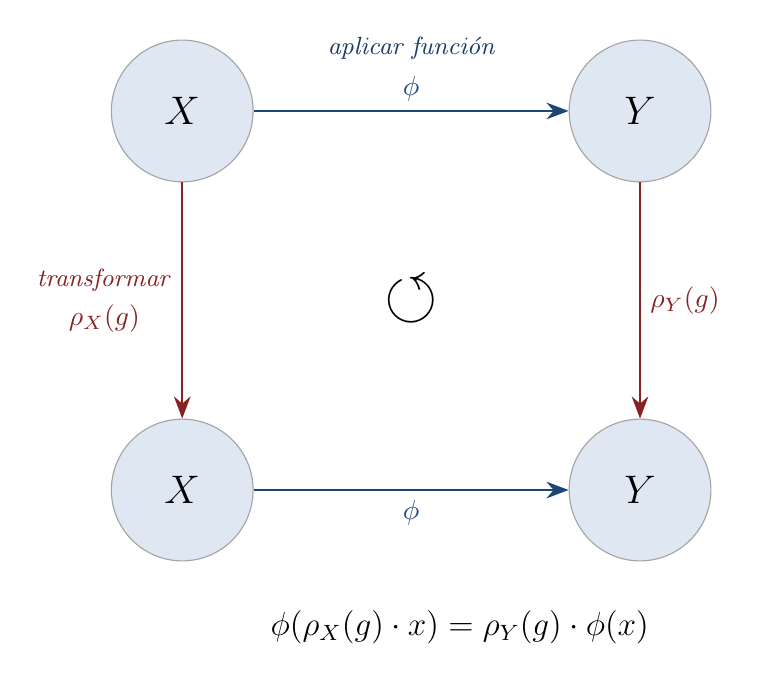
\begin{tikzpicture}[
    node distance=3cm and 4cm,
    space/.style={circle, draw=gdlgray!80, fill=gdlblue!15, minimum size=1.8cm, font=\Large},
    arrow/.style={-{Stealth[length=8pt]}, thick},
    label/.style={font=\normalsize, midway}
]

% Los cuatro nodos del diagrama conmutativo
\node[space] (X) {$X$};
\node[space, right=of X] (Y) {$Y$};
\node[space, below=of X] (gX) {$X$};
\node[space, below=of Y] (gY) {$Y$};

% Flechas horizontales (función φ)
\draw[arrow, gdlblue!70!black] (X) -- node[label, above] {$\phi$} (Y);
\draw[arrow, gdlblue!70!black] (gX) -- node[label, below] {$\phi$} (gY);

% Flechas verticales (acción del grupo)
\draw[arrow, gdlred!70!black] (X) -- node[left, align=center] {\small\textit{transformar}\\[2pt] $\rho_X(g)$} (gX);
\draw[arrow, gdlred!70!black] (Y) -- node[label, right] {$\rho_Y(g)$} (gY);

% Etiquetas de los caminos
\node[font=\small\itshape, gdlblue!60!black] at ($(X)!0.5!(Y) + (0,0.8)$) {aplicar función};

% Símbolo de conmutatividad
\node[font=\Huge] at ($(X)!0.5!(gY)$) {$\circlearrowleft$};

% Ecuación de equivarianza
\node[font=\large, below=0.5cm of gX, anchor=north west, xshift=1cm] {
    $\phi(\rho_X(g) \cdot x) = \rho_Y(g) \cdot \phi(x)$
};

\end{tikzpicture}
\end{document}
